\section{Viscous Friction}

The goal of this test is to determine the viscous friction depending on the velocity, meaning the torque that is needed to maintain a constant velocity. This is also needed to compare the transparency of the different devices. In order to calculate the viscous friction we have to use the following equation:

\begin{equation}
    Inertia * \ddot\theta = \tau_{motor} - \tau_{visc} = k_{t}*i_{meas} -\tau_{visc}
\end{equation}

with $k_{t}$ being the torque constant and $i_{meas}$ being the motor current. We only investigate steady states after a constant velocity is reached and the acceleration is zero. Therefore we can calculate the viscous friction as follows:

\begin{equation}
    \tau_{visc} = k_{t}*i_{meas}
\end{equation}

\subsection{Implementation}

We want to measure the torque produced by the motor while a constant velocity is maintained. Therefore, the robot needs to move with a desired constant velocity, this is especially difficult because our range of motion is relatively small. The desired velocity can be set by setting a desired distance and a desired duration in which the distance has to be overcome. For example if you wish to have 200 $\frac{deg}{s}$ you could set a distance of 200° and a duration of 1s. It is best to have a distance as large as possible or else large velocities will be difficult to maintain. I always took 200° and started at the mechanical stop. The measurement has to be taken separately for each velocity. Also the data analysis can only be done for one velocity at a time, so it is not automatically done.

\subsection{Data Analysis}

For the data analysis, the measured current as well as the velocity are recorded over time and written to a tdms file. As mentioned before, one tdms file is generated for each velocity and they also have to be analysed separately. The two signals can be plotted over time. Afterwards one has to determine a section of the signals where the velocity is as constant as possible, this has to be done visually. One can then calculate the average consumed current over this section and calculate the viscous friction. 

\subsection{Results}

The results for MIKE 3 and MIKE 6 are depicted in the following plots:

\begin{figure}[h]
    \begin{minipage}[m]{0.48\textwidth}
     \centering
        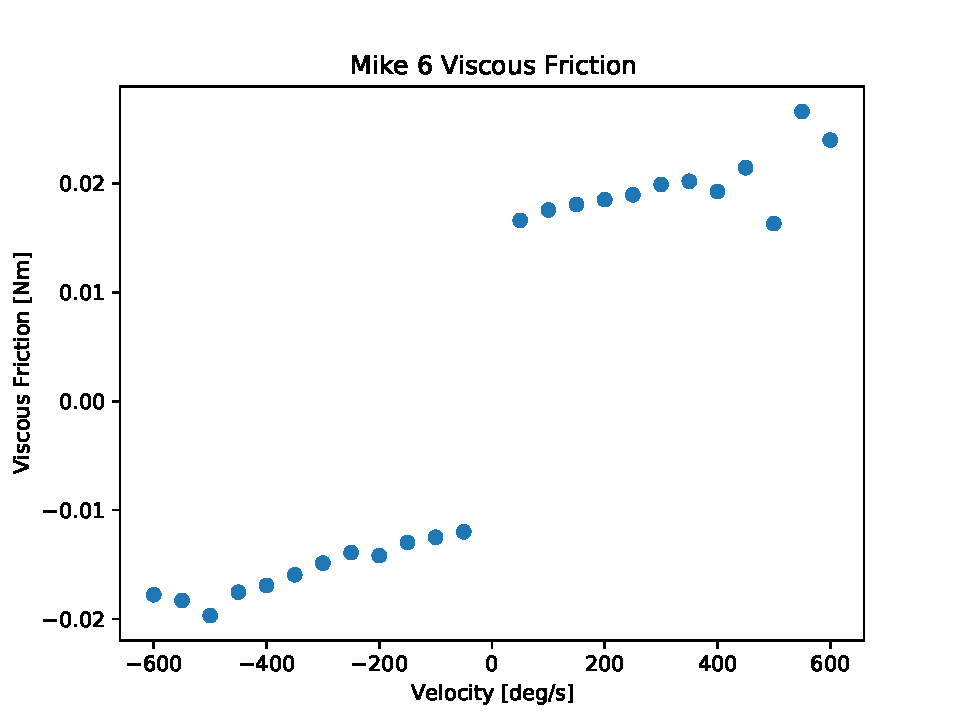
\includegraphics[width = \textwidth]{chapters/dynamic friction/Mike6_DynamicFriction.pdf}
    \end{minipage}
    \hfill
    \begin{minipage}[m]{0.48\textwidth}
     \centering
        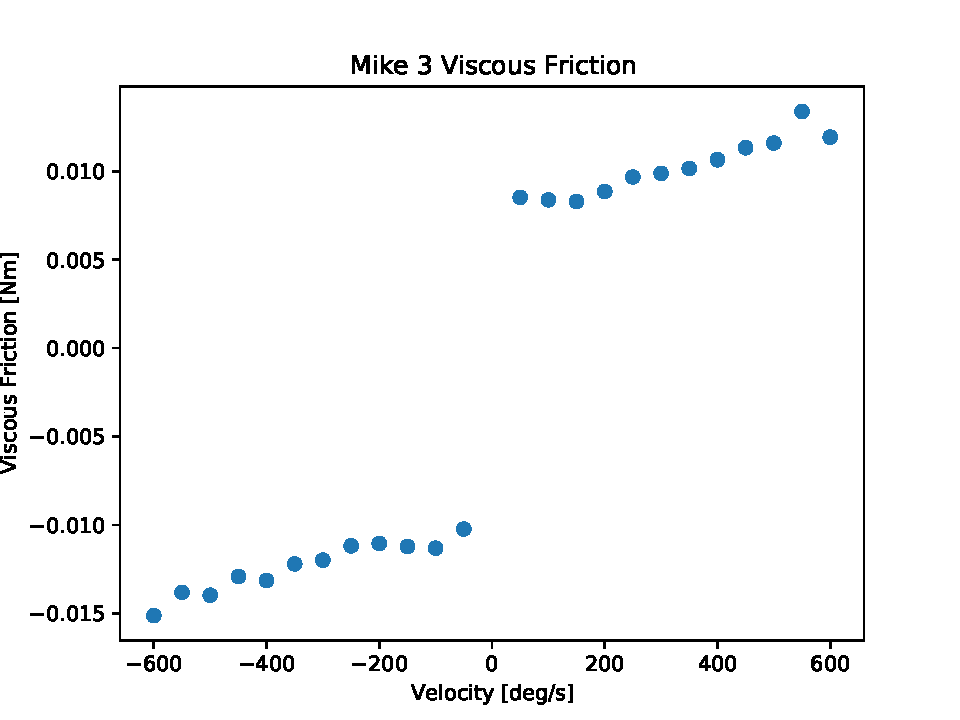
\includegraphics[width = \textwidth]{chapters/dynamic friction/Mike3_DynamicFriction.pdf}
    \end{minipage}
\end{figure}

It is visible that the viscous friction increases with higher velocities, which was also observed in Monika's ICORR paper and Julian's report. The measurements of the different MIKE versions are close to each other, again MIKE \#3 seems to have less friction, which was also observed in the static friction. The obtained results are also similar to Monika's ICORR paper and Marc's final report. The observed values were $<0.04Nm$ (Monika's ICORR paper \cite{icorr}) and $<0.02Nm$ (Marc's Report \cite{marc}).